\documentclass[12pt]{article}
\usepackage[top=1in,bottom=1in,left=1in,right=1in]{geometry}
\usepackage{alltt}
\usepackage{array}	
\usepackage{graphicx}
\usepackage{tabularx}
\usepackage{verbatim}
\usepackage{setspace}
\usepackage{listings}
\usepackage{amssymb,amsmath, amsthm}

\title{SOEN331: Introduction to Formal Methods\\for Software Engineering\\
Assignment 2 on Extended Finite State Machines}
\author{Author's name}
\date{\today}

\begin{document}
\begin{spacing}{1.5}

\maketitle

\section{Metro passageway formal specification}

\noindent The EFSM of the metro passageway is the tuple $S = (Q, \Sigma_1, \Sigma_2, q_0, V, \Lambda)$, where\\

\noindent $Q = \{locked, unlocked\}$\\
\noindent $\Sigma_1 = \{request~entry, pass\}$\\
\noindent $\Sigma_2 = \{lock, unlock, beep\}$\\
\noindent $q_0: locked$\\
\noindent $V: ticket = \{valid, invalid\}$\\
\noindent $\Lambda$: Transition specifications\\
\indent 1. $\rightarrow locked$\\
\indent 2. $locked \xrightarrow {\text { request entry [ticket is valid] / (unlock ; beep)}} unlocked$\\
\indent 3. $unlocked \xrightarrow {\text { pass / lock}} locked$\\

\noindent The UML state diagram is shown in Figure~\ref{fig:metro-fig}.

\newpage

\section{UML state diagrams}

\begin{figure}[h!]
	\centering
		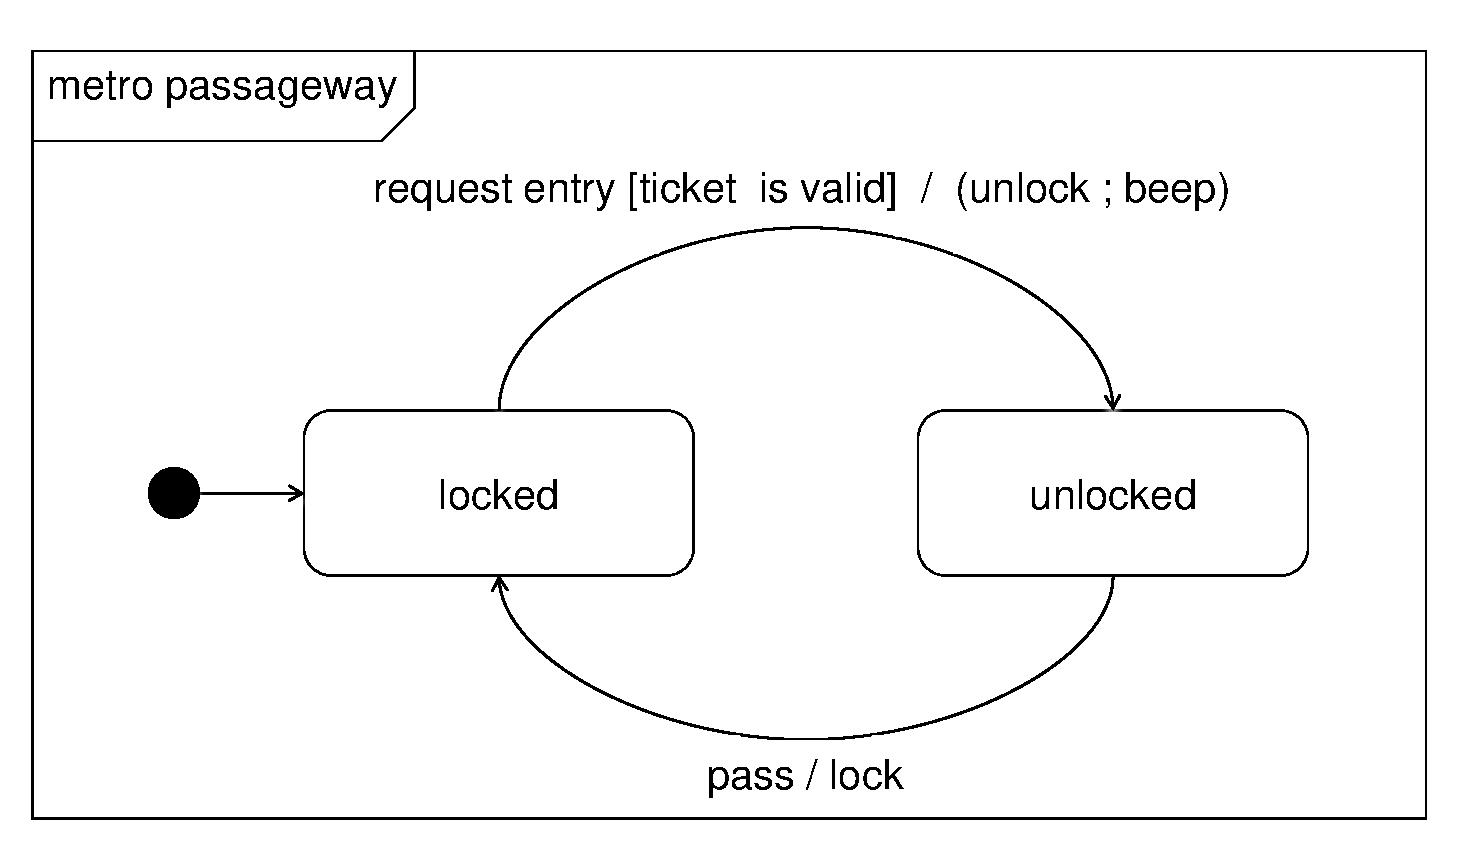
\includegraphics[width=0.8\textwidth]{./figures/eps/metro.eps}
		  \caption{Metro.}
  \label{fig:metro-fig}
\end{figure}

\end{spacing}


\end{document}
